\documentclass{beamer}
\usepackage[utf8]{inputenc}

\usetheme{Madrid}
\usecolortheme{default}

%------------------------------------------------------------
%This block of code defines the information to appear in the
%Title page
\title[Final Report] %optional
{Final Report of the Guide Study (CS6534)}

\subtitle{Topic: Physical layer key generation for wireless sensor networks}

\author[HUANG Kunlun] % (optional)
{HUANG Kunlun}


\institute[CityU HK] % (optional)
{
  {Supervisor:}

  {Professor XU Weitao}
  \and
  Department of Computer Science\\
  City University of Hong Kong
  
}

\date[Guide Study Presentation] % (optional)
{Guide Study Presentation, December 2023}

\logo{
\includegraphics[height=1cm]{cityulogo}}

%End of title page configuration block
%------------------------------------------------------------



%------------------------------------------------------------
%The next block of commands puts the table of contents at the 
%beginning of each section and highlights the current section:

\AtBeginSection[]
{
  \begin{frame}
    \frametitle{Table of Contents}
    \tableofcontents[currentsection]
  \end{frame}
}
%------------------------------------------------------------


\begin{document}

%The next statement creates the title page.
\frame{\titlepage}


%---------------------------------------------------------
%This block of code is for the table of contents after
%the title page
\begin{frame}
\frametitle{Table of Contents}
\tableofcontents
\end{frame}
%---------------------------------------------------------


\section{Introduction}

%---------------------------------------------------------
%Changing visivility of the text
\begin{frame}
\frametitle{Introduction}
\textbf{Vital:}

Network security is a recent scorching topic and affects everyone's vital interests. PKI-based password management systems such as SSL and TLS are regarded as an excellent way to solve the problem of encrypted communication in computer networks. \pause 
\begin{figure}
  \centering
  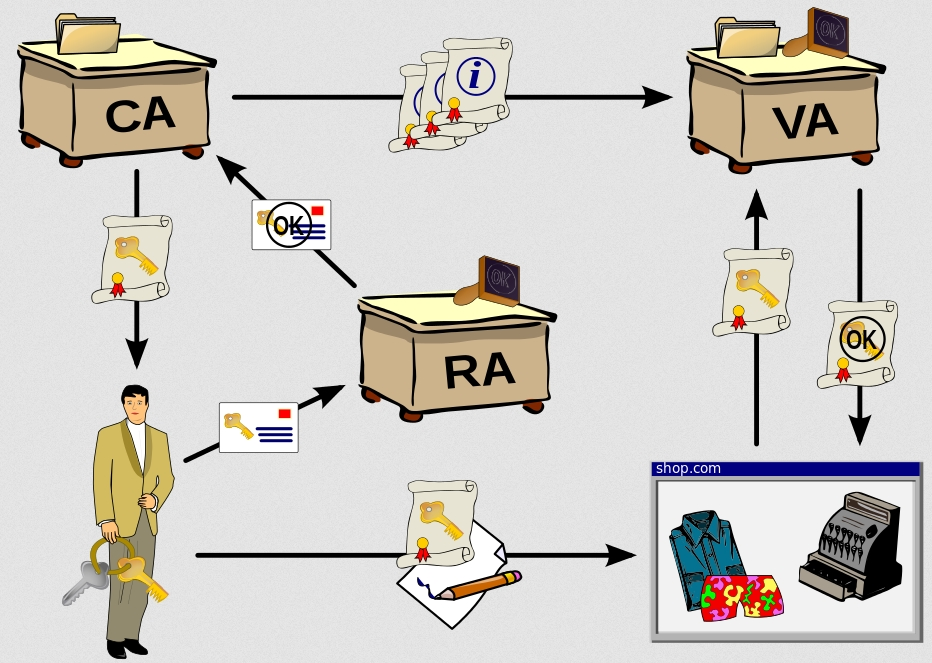
\includegraphics[width=0.4\linewidth]{figures/pkisystem.png}
  \caption{PKI System\cite{wiki:Public_key_infrastructure}}
  \label{fig:pkisystem}
\end{figure}
OK?
\end{frame}

\begin{frame}
\frametitle{Introduction}
\begin{alertblock}{Not Suitable}
  However, in the field of the Internet of Things(IoT), due to issues such as node computing performance and the difficulties in key management in large amount of nodes, PKI systems are \textbf{not suitable} in it. 

\end{alertblock}
\vspace{0.05in}
\end{frame}

\begin{frame}
  \frametitle{Introduction}
\textbf{Rapid Growing of IoT Market:}

According to Gartner\cite{gartnerresearchiot}, there will be over 43 billion IoT devices connected to the internet by 2023, and the IoT market size will reach US\$1.4 trillion. The rapid development of the IoT is mainly due to the following trends. Also, the MIIT suggests that the IoT is a future development trend that will have a profound impact on all industries\cite{iot13th5yr}. 

\begin{figure}
  \centering
  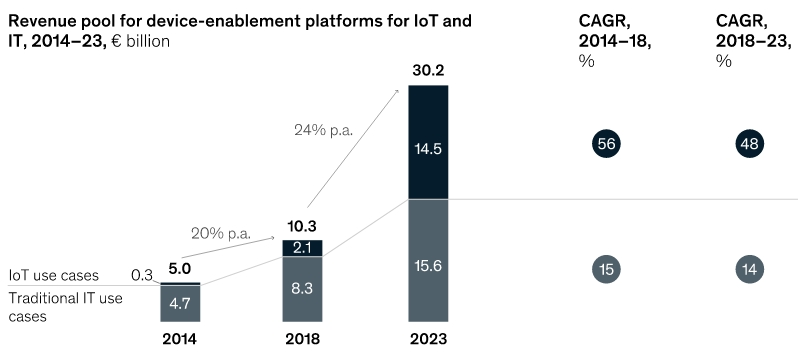
\includegraphics[width=0.7\linewidth]{figures/iotgrowing.png}
  \caption{IoT Growing\cite{Dahlqvist_Patel_Rajko_Shulman_2019}}
  \label{fig:iotgrowing}
\end{figure}

\end{frame}

%---------------------------------------------------------


%---------------------------------------------------------
\begin{frame}
\frametitle{Introduction}

To address this problem, \textbf{Physical layer key generation(PLKG)} have been proposed. Which is a technique for generating cryptographic keys from the physical characteristics of a wireless communication channel. This can be done by exploiting the unique features of the channel, such as its fading characteristics, noise properties, and path loss. \pause
\begin{block}{Attractive}
  PLKG particularly attractive for wireless sensor networks (WSNs) because it does not require any prior shared information between the nodes, and it can be implemented with relatively low computational overhead.
\end{block}

\end{frame}

\begin{frame}
\frametitle{Introduction}
  
Physical layer key generation has recently been a research hotspot in academia and industry\cite{7120014}, focuses only on traditional wireless  technologies such as Wi-Fi, ZigBee, and 5G Radio Access Network. 

In the area of Low-Power Wide-Area Networks (LPWAN)\cite{iotfactorylpwan}, the \textbf{long communication distance, low power consumption, and low trans rate} bring new research challenges to physical layer key generation.
  
  \begin{figure}
    \centering
    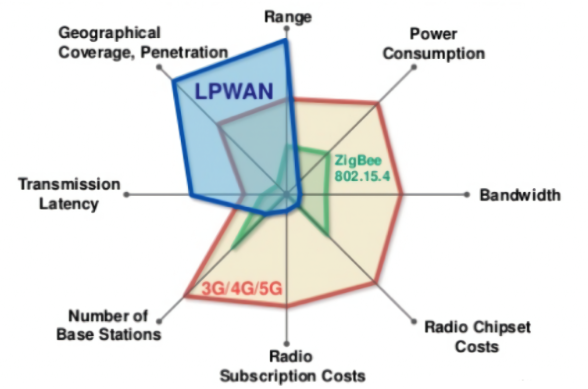
\includegraphics[width=0.42\linewidth]{../figures/fig1-1.png}
    \caption{LPWAN vs. Other wireless communication technologies\cite{iotfactorylpwan}}
    \label{fig:1-1}
  \end{figure}
\end{frame}

\begin{frame}
  \frametitle{Sample frame title}
  
  In this slide, some important text will be
  \alert{highlighted} because it's important.
  Please, don't abuse it.
  
  \begin{block}{Remark}
  Sample text
  \end{block}
  
  \begin{alertblock}{Important theorem}
  Sample text in red box
  \end{alertblock}
  
  \begin{examples}
  Sample text in green box. The title of the block is ``Examples".
  \end{examples}
  \end{frame}

%---------------------------------------------------------

\section{Related Work}

%---------------------------------------------------------
%Highlighting text
\begin{frame}
\frametitle{Related Work - Physical Layer Key Generation}
Generally, physical layer key generation applies the following five steps to generate a key: channel probing, randomness extraction, quantization, information reconciliation, and privacy amplification\cite{7120014}.
\begin{figure}
  \centering
  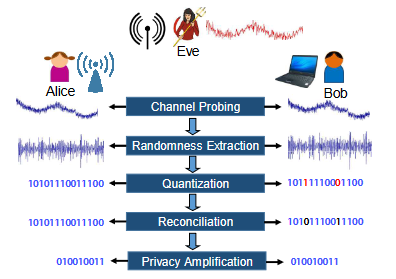
\includegraphics[width=0.6\linewidth]{../figures/fig2-1.png}
  \caption{Physical Layer key Generation Model\cite{7120014}}
  \label{fig:phykegen}
\end{figure}

\end{frame}
%---------------------------------------------------------


%---------------------------------------------------------
%Two columns
\begin{frame}
\frametitle{Two-column slide}

\begin{columns}

\column{0.5\textwidth}
This is a text in first column.
$$E=mc^2$$
\begin{itemize}
\item First item
\item Second item
\end{itemize}

\column{0.5\textwidth}
This text will be in the second column
and on a second tought this is a nice looking
layout in some cases.
\end{columns}
\end{frame}
%---------------------------------------------------------

\section{Project Outline and Methodology}

%---------------------------------------------------------
%Example of the \pause command
\begin{frame}
In this slide \pause

the text will be partially visible \pause

And finally everything will be there
\end{frame}
%---------------------------------------------------------

\section{System modeling and Implementation}

%---------------------------------------------------------
%Example of the \pause command
\begin{frame}
In this slide \pause

the text will be partially visible \pause

And finally everything will be there
\end{frame}
%---------------------------------------------------------



\section{Conclusion}

%---------------------------------------------------------
%Example of the \pause command
\begin{frame}
In this slide \pause

the text will be partially visible \pause

And finally everything will be there
\end{frame}
%---------------------------------------------------------

\appendix
\begin{frame}
\bibliographystyle{ieeetr} % 
\bibliography{refs} % Entries are in the refs.bib file
\end{frame}

\end{document}